\documentclass[twocolumn]{article}
\usepackage[utf8]{inputenc}

\usepackage{mathtools}
\usepackage{hyperref}
\hypersetup{
    colorlinks=true,
    linkcolor=blue,
    filecolor=magenta,      
    urlcolor=cyan,
}

\title{Actividad 4}
\author{Miguel Terán}
\date{14 de septiembre de 2021}

\begin{document}




\maketitle
\section{Medición de tiempos de procesado}
\subsection{Programa \texttt{trap}.}

Para esta actividad se procedió a ejecutar el programa \texttt{trap} con diferentes números de procesos. Los \textit{nodos} que se utilizaron fueron: \textit{cero, uno, tres, cinco, seis, siete, ocho, nueve, diez, once, doce, trece, catorce} y \textit{quince}, es decir, solo se utilizaron $14$ nodos. Ello, debido a fallas técnicas presentadas a la hora de realizar las mediciones. Los nodos utilizados permitió ejecutar el programa hasta con un número de procesos máximo de $56$.

En la figura \ref{fig1} se puede observar los datos recopilados para los tiempos \textit{real}, \textit{user} y \textit{sys}, los cuales son el producto de un promedio de tres series de mediciones para cada categoría de tiempo. Se puede apreciar en la figura que los datos muestran un comportamiento lineal con pendiente positiva. Esto, significa que el tiempo de procesado del programa en ejecución aumenta con respecto al número de procesos.

En la figura \ref{fig2} se muestra un promedio de los tiempos \textit{real}, \textit{user} y \textit{sys}. Esto, para tener una perspectiva general del tiempo de procesado del programa ejecutado en cuestión. En esta gráfica se puede observar dos regiones. La primera región que está entre $1$ y $10$ número de procesos, se puede observar un comportamiento lineal, pero con una pendiente muy pronunciada. Por otro lado, en la segunda región que está entre $10$ y $56$ se observa un comportamiento relativamente estable, pero con un patrón de crecimiento en el tiempo a medida que el número de procesos aumenta. 


\begin{figure}
    \centering
    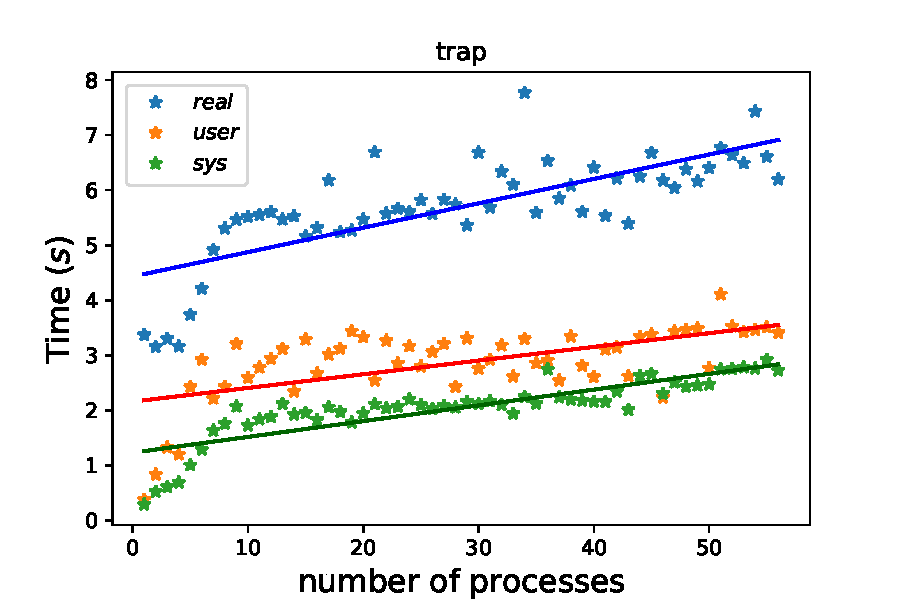
\includegraphics[width=3in]{fig_1.pdf}
    \caption{Se muestra los datos correspondientes a los tiempos \textit{real}, \textit{user} y \textit{sys}. Asimismo, en la gráfica se muestra los ajustes lineales correspondientes para cada conjunto de datos. La línea azul corresponde a la ecuación: $t_1=0.044*np + 4.431$, la línea roja corresponde a la ecuación: $t_2=0.024*np + 2.159$ y la línea verde corresponde a la ecuación: $t_3 = 0.028*np + 1.232$.} \label{fig1}
\end{figure}

\begin{figure}
    \centering
    \includegraphics[width=3in]{timeProcesses2.pdf}
    \caption{Se muestra un promedio de los tiempos \textit{real}, \textit{user} y \textit{sys}. La línea azul corresponde a la ecuación: $t =0.032*np + 2.607$. } \label{fig2}
\end{figure}

\subsection{Programas \texttt{trap\_Gdata} y \texttt{trap\_Gdata1}.}

Se procedió a modificar el programa \texttt{trap}. En una segunda versión se le agregó al código la opción de que los datos del programa puedan ser otorgados por el usuario, a esta versión se le dio el nombre de \texttt{trap\_Gdata}. Posteriormente, se mejoro el código distribuyendo el \texttt{Input} del programa a través de un \textit{árbol de procesos}. Esta forma de distribuir el \texttt{Input} reduce los pasos para transmitir la información en función de los $p$ procesos. A este último programa se le dio el nombre de \texttt{trap\_Gdata1.}

En la figura \ref{fig3} se puede observar que existe mucha dispersión en los datos correspondientes a el tiempo \textit{user}. Esto, se debe a que el \texttt{Input} es dado por el usuario, lo cual conlleva cierto ruido en la medición del tiempo. Por otra parte, la gráfica correspondiente al tiempo \textit{real} muestra un cambio en la tendencia, es decir, posee una pendiente negativa $m=-0.018$. Dicho con otras palabras, el tiempo de procesado disminuye en función del \textit{número de procesos}. Finalmente, el tiempo \textit{sys} se observa muy atenuada pero con una tendencia ligeramente positiva.

\begin{figure}
    \centering
    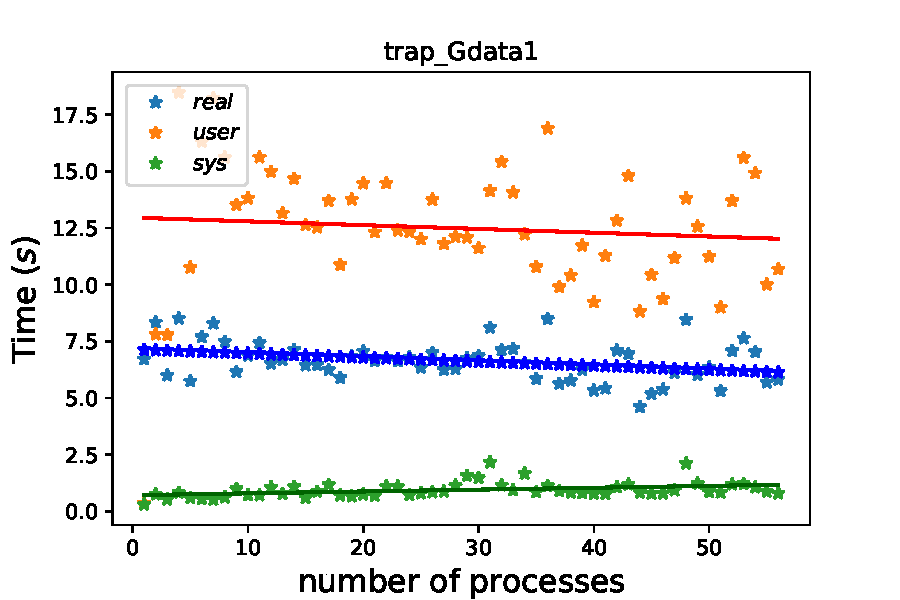
\includegraphics[width=3in]{fig_3.pdf}
    \caption{Se muestra los tiempos obtenidos al copilar el programa \texttt{trap\_Gdata1} con el \texttt{Input}: $a=0$, $b=1$ y $n=1024$. La línea ($*$) azul corresponde a la ecuación: $t =-0.018*np + 7.15$. La línea roja es: $t = -0.016*np + 12.962$. Finalmente, la línea verde es: $t = 0.008*np + 0.716$. } \label{fig3}
\end{figure}

\subsection{Programa \texttt{trap\_Gdata2}.}

Se mejoró el programa \texttt{trap\_Gdata1} aprovechando las funciones predefinidas que posee el protocolo \texttt{MPI}. Se empleó la función \texttt{MPI\_Bcast}, la cual envía un mensaje con los datos del \texttt{Input} desde el \texttt{rank root} a todos los procesos del grupo.

En la figura \ref{fig4} se puede apreciar que tiene características similares a la figura \ref{fig3}. Se observa que la gráfica correspondiente al tiempo \textit{real} obedece a una  recta con pendiente negativa $m=-0.012$. Ello, conlleva a que el tiempo de procesado disminuye con respecto al número de procesos.

En la figura \ref{fig5} se aprecia una comparación de los tiempos \textit{real} observados en las figuras \ref{fig1}, \ref{fig3} y \ref{fig4}. Se puede apreciar que el programa \texttt{trap} es ineficiente al procesarlo en paralelo. Por otra parte, los programas \texttt{trap\_Gdata1} y \texttt{trap\_Gdata2} obtienen una disminución en el tiempo de procesado. Asimismo, se puede observar que el programa que arroja mejores resultados es \texttt{trap\_Gdata2}. Sin embargo, el programa \texttt{trap\_Gdata1} presenta una pendiente negativa más pronunciada que la del programa \texttt{trap\_Gdata2}. 

\begin{figure}
    \centering
    \includegraphics[width=3in]{fig_Broadcast.pdf}
    \caption{Se muestra los tiempos obtenidos al copilar el programa \texttt{trap\_Gdata2} con el \texttt{Input}: $a=0$, $b=1$ y $n=1024$. La línea ($+$) azul corresponde a la ecuación: $t =-0.012*np + 6.011$. La línea roja es: $t =-0.015*np + 10.498$. Finalmente, la línea verde es: $t = 0.004*np + 0.763$. } \label{fig4}
\end{figure}

\begin{figure}
    \centering
    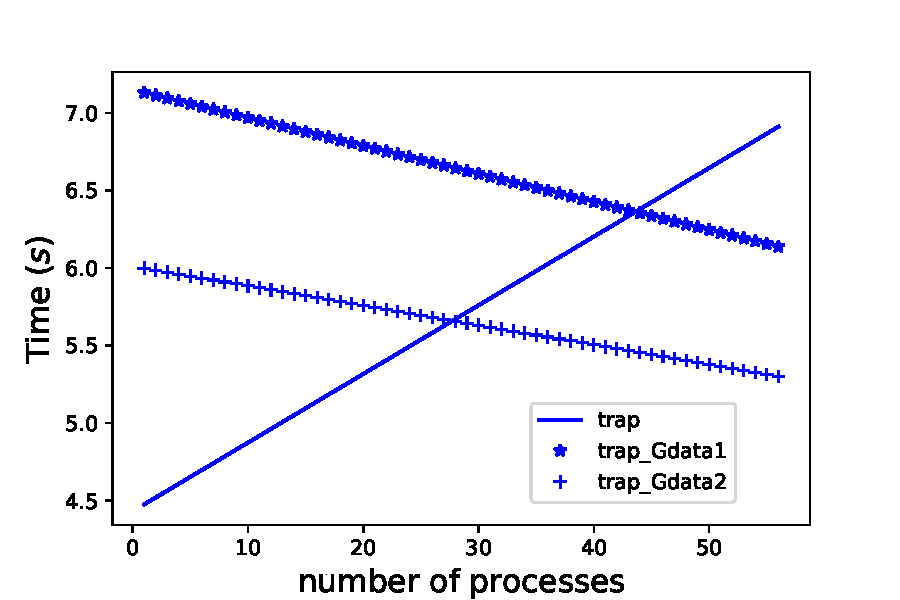
\includegraphics[width=3in]{fig_5.pdf}
    \caption{Se muestra una comparación de los tiempos \textit{real} para cada caso.} \label{fig5}
\end{figure}

\section{Conclusiones}
Se pudo observar que aunque el programa \texttt{trap} es compatible con la programación en paralelo, para este caso no es viable bajo los parámetros establecidos. El tiempo de procesado aumentó a medida que se utilizaron más procesadores. Ello, se puede adjudicar posiblemente al costo de tiempo de la comunicación entre los \textit{nodos}. 

Se apreció que las modificaciones introducidas en los programas \texttt{trap\_Gdata1} y \texttt{trap\_Gdata2} produjeron un cambio en la tendencia de los tiempos de procesado. Dicho con otras palabras, los tiempos de procesado  estadísticamente disminuyeron en función del número de procesos. El programa que arrojó mejores resultados fue \texttt{trap\_Gdata2}. Sin embargo, la tendencias mostradas en los resultados muestran que posiblemente el programa \texttt{trap\_Gdata1} sea el mejor para números muy grandes de procesado. 

\end{document}

